
\section{SECDA-DSE}
\label{method}

SECDA-DSE extends the SECDA ecosystem by introducing an LLM-guided framework for accelerator DSE. The framework combines a structured DSE with reasoning-guided refinement to iteratively generate, evaluate, and improve accelerator configurations for target workloads and FPGA platforms.

The SECDA-DSE workflow is shown in Figure~\ref{fig:SECDA-DSE}. It takes as input: (i) a target workload (e.g., CNNs, DNNs); (ii) a target FPGA device; and (iii) architectural directives that constrain or guide architecture exploration, such as tiling parameters, compute parallelism, and memory hierarchy organization. Based on these inputs, SECDA-DSE generates SECDA native accelerator designs, evaluates them through simulation and hardware execution flows, and stores the resulting hardware datapoints for future refinement iterations.


\begin{figure}[!tb]
  \centering
  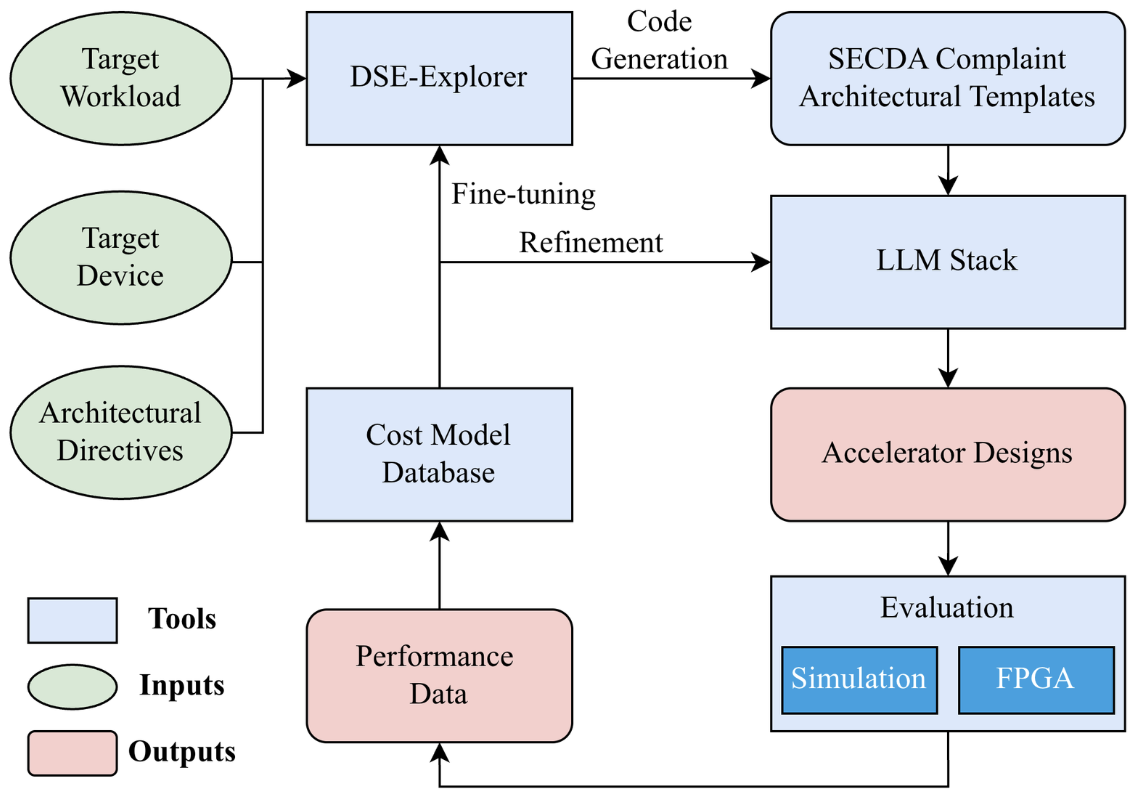
\includegraphics[width=0.95\linewidth]{img/SECDA-DSE.png}
  % \caption{SECDA-DSE framework architecture showing the interaction between the DSE Explorer and the LLM Stack.}
  \caption{SECDA-DSE workflow showing the interaction between the DSE Explorer, LLM Stack, and Evaluation Module.}
  \label{fig:SECDA-DSE}
\end{figure}


Unlike unconstrained hardware generation approaches, SECDA-DSE operates within the SECDA ecosystem using template-constrained accelerator generation.
While constrained limits exploration to SECDA-compliant architectural patterns, it enables the reliable generation of synthesizable and executable accelerators while still allowing the LLM Stack to explore a large design space encompassing compute parallelism, memory organization, and dataflow configurations. 
%In addition, it achieves self-improvement through reasoning about errors encountered in initial design generations. 
Furthermore, the framework iteratively refines generated designs by reasoning about errors identified in earlier iterations.

% and accelerator-small point in the presentation. 
%Action1.1 
%- N/Asmall point in the presentation. 
%Action1.1 
%- N/Aspecific architectural refinements. 


%******************************************************************************************************

\subsection{DSE Explorer}

The DSE Explorer is responsible for structured exploration of the accelerator design space. Its primary role is to generate candidate accelerator configurations under workload and FPGA-specific constraints. 

The DSE Explorer operates by generating permutations of architectural parameters, including compute unit dimensions, tiling strategies, buffer allocations, and dataflow configurations. These parameter sets are instantiated into SECDA-compliant accelerator templates, enabling integration with existing SECDA simulation and FPGA execution flows. 
Each generated accelerator configuration produces an individual design run consisting of the accelerator description, generated source files, HLS outputs, and FPGA execution artifacts. The resulting hardware design is evaluated using SECDA-based simulation and downstream synthesis flows to collect performance metrics including execution latency, resource utilization, and data movement costs.

These evaluation outputs are stored as hardware datapoints that are later re-used to fine-tune the LLM Stack and guide subsequent refinement iterations. By combining structured parameter exploration with evaluation-driven feedback, the DSE Explorer enables SECDA-DSE to navigate large accelerator design spaces more efficiently than exhaustive exploration approaches.


%******************************************************************************************************

\subsection{LLM Stack}

The LLM Stack acts as the reasoning and orchestration layer within SECDA-DSE. Its role is to analyze the generated accelerator configurations, reason about hardware trade-offs, and guide exploration refinement across iterations. 
It incorporates RAG, CoT prompting, and parameter-efficient fine-tuning to provide workload-aware accelerator design generation. Figure~\ref{fig:LLM_STACK} provides a high-level overview of the complete LLM Stack and interaction between components and across the modules.


\begin{figure}[!tb]
  \centering
  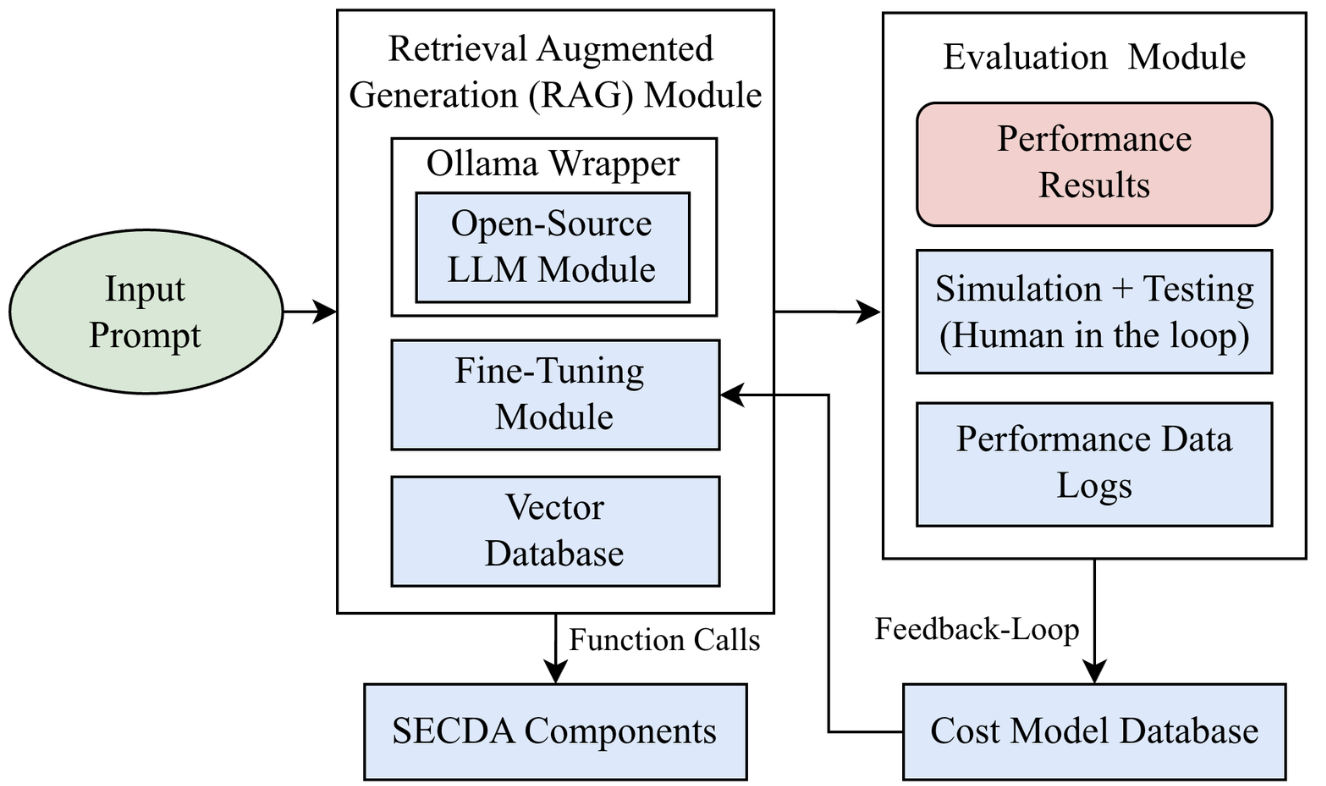
\includegraphics[width=0.95\linewidth]{img/LLM_STACK.png}
  \caption{Overview of LLM Stack Architecture.}
  \label{fig:LLM_STACK}
\end{figure}



\subsubsection{Retrieval-Augmented Generation}
The RAG module enables the LLM Stack to retrieve contextual information from a vectorized SECDA knowledge-base consisting of SECDA-TFLite source code, architectural templates, API-level context, and previously evaluated hardware datapoints. 
Rather than exposing the complete SECDA codebase or full hardware logs during each iteration, the RAG module retrieves only the most relevant code fragments and hardware summaries associated with the current exploration step. We employ a graph-based retrieval approach to efficiently identify relevant code context, using fuzzy matching on code comments to guide navigation across graph nodes. This method reduced retrieval overhead compared to standard nearest-neighbor retrieval approaches while improving contextual relevance during generation. 
% This method provided approximately 1.8$\times$ speedup compared to default techniques such as k-nearest neighbor search, and thus reduces the overall design generation time. 

This retrieval-based approach enables SECDA-DSE to maintain manageable context sizes while still providing sufficient architectural context for refinement. The retrieved information includes workload characteristics, prior accelerator configurations, hardware utilization summaries, and evaluation outcomes, before recommending new design configurations.


\subsubsection{Chain-of-Thought Prompting and Fine-Tuning}
SECDA-DSE employs CoT prompting to encourage structured multi-step reasoning during accelerator exploration. CoT prompts enable the LLM Stack to reason about workload behavior, hardware constraints, memory organization, and compute parallelism before generating candidate architectural refinements.

For model adaptation, SECDA-DSE uses parameter-efficient fine-tuning with LoRA~\cite{hu2022lora}. The fine-tuning dataset is built using previously explored accelerator configurations and their associated hardware evaluation outcomes generated via DSE-Explorer, with a human-in-the-loop for ensuring correctness.

Each hardware datapoint consists of workload and FPGA context, generated architectural configuration, simulation and execution success status, execution latency, and resource utilization metrics. These datapoints enable the LLM Stack to iteratively adapt toward generating configurations that are feasible, performance-aware, and target-device-aware.


%******************************************************************************************************

\subsection{Evaluation and Feedback Loop}

The Evaluation Module is responsible for validating generated accelerator designs and collecting feedback used for iterative refinement. The workflow begins with a SECDA-based SystemC simulation to verify functional correctness and collect early-stage performance estimates. Generated accelerator designs are then passed through HLS and once succeed go through FPGA execution flows. 
The collected evaluation metrics include execution latency, FPGA resource utilization, DMA transfer characteristics, data movement costs, and hardware execution validation. These results are stored within the SECDA-DSE hardware datapoint database and reused during subsequent exploration iterations.

To reduce invalid accelerator proposals, SECDA-DSE constrains generation using SECDA native architectural templates and device-aware parameter ranges rather than relying on unconstrained free-form hardware generation. Candidate designs that fail simulation, violate resource constraints, or fail downstream synthesis flows are rejected and logged as negative datapoints, which are again fed back as a negative reinforcement to the LLM to reason and correct.

The iterative interaction between the DSE Explorer, LLM Stack, and Evaluation Module enables SECDA-DSE to repeatedly refine accelerator exploration decisions while leveraging prior hardware evaluation knowledge across workloads and FPGA platforms. 

% As of now, as the work is still in its initial phases, we are having a human in the loop performing the testing and logging the error.